\section{Filter}
Wenn Filter symetrisch sind, ist die Phase konstant mit einem $\frac{n}{2}$ Verzögerung. 

\subsection{PID}
\[
H(z) = P + \frac{I}{1 - z^{-1}} + D(1-z^{-1})
\]
\begin{center}
	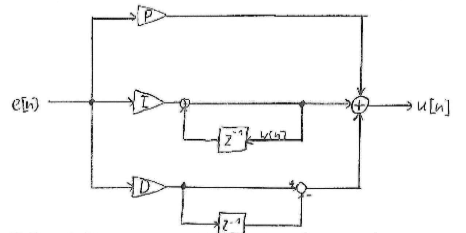
\includegraphics[width=0.7\columnwidth]{Images/pid}
\end{center}

\subsection{Design Filter}
\subsubsection{Low Pass}\script{S242}
Das Verhältniss muss bei einem Low-Pass Filter $H(z)$ erster Ordnung kleiner als 1 sein.
\[
H(z) = \frac{G(1 + bz^{-1})}{1 - az^{-1}}
\]

Damit ergibt sich eine Geleichung:
\[
\frac{H(\pi)}{H(0)} = \frac{(1 - b)(1 - a)}{(1+ b)(1 +a)}
\]
Mit einer zweiten Gleichung, kann nun der Filter desigend werden. Debei wird zB festgelegt, dass der Filter innerhalb von $n_{eff} = 20$ Samples, 1\% ($\epsilon=0.001$) vom Steady State erreichen muss.
\[
a = \epsilon^{\frac{1}{n_{eff}}} = 0.01^{\frac{1}{20}} = \approxeq 0.8
\]
Mit der Gleichung oben, kann nun auch $b$ berechnet werden. Der Faktor $G$ kann nicht mittels Pole/Zero Plot gefunden werden!

\begin{center}
	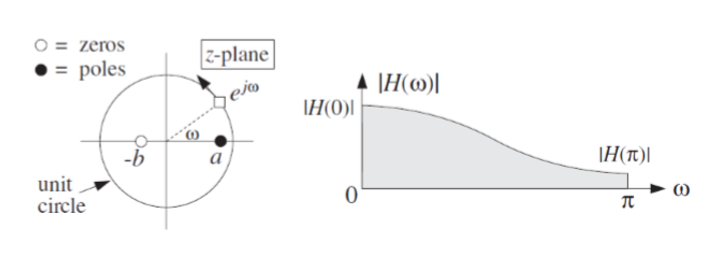
\includegraphics[width=0.8\columnwidth]{Images/lp}
\end{center}

\subsubsection{Resonators}\label{sec:resonators}\script{S244}
Filter $H(z)$ mit conjugiert-complexem Pol $p = Re^{\pm j\omega_0}$ nahe am Einheitskreis mit $\omega_0 = \frac{2\pi f_0}{f_s}$
\[
H(z) = \frac{G}{(1-pz^{-1})(1-p^*z^{-1})} = \frac{G}{1+a_1z^{-1}+a_2z^{-2}}
\]

Mit den Voraussetzungen $0\gt R\gt 1$ und $0\gt \omega_0 \gt \pi$ lassen sich die Koeffizieten bestimmen:
\[
a_1 = -2R\cos(\omega_0), \qquad a_2 = R^2
\]

Hier wird $G$ oft mit $\left|H(\omega_0)\right| = 1$ normiert.
\[
G = (1-R)\sqrt{1-2R\cos(2\omega_0)+R^2}
\]

Die Breite $\Delta\omega \approxeq 2(1-R)$ kann mit bestimmt werden. Oft wird diese Formel für das definieren von der Variable \textbf{R} verwendet um anschliessend die Koeffizieten zu bestimmen.

\begin{center}
	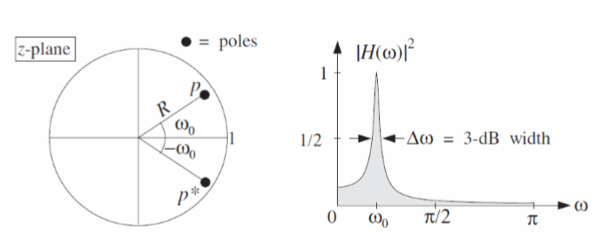
\includegraphics[width=0.8\columnwidth]{Images/resonator}
\end{center}


\subsubsection{General Resonators}
Durch einsetzen von Zeros $b = re^{\pm j\omega_0}$ auf der selben Achse wie die Pole in \ref{sec:resonators} können weitere Filter $H(z)$ entwickelt werden.
\[
H(z) = \frac{(1-bz^{-1})(1-b^*z^-1)}{(1-pz^{-1})(1-p^*z^{-1})} =  \frac{1+b_1z^{-1}+b_2z^-2}{1+a_1z^{-1}+a_2z^{-2}}
\]
Mit den Voraussetzungen $0\gt r\gt 1$ lassen sich die Koeffizieten bestimmen:
\begin{align*}
	b_1 = -2r\cos(\omega_0), &\qquad b_2 = r^2 \\
	a_1 = -2R\cos(\omega_0), &\qquad a_2 = R^2 \\
\end{align*}

\begin{center}
	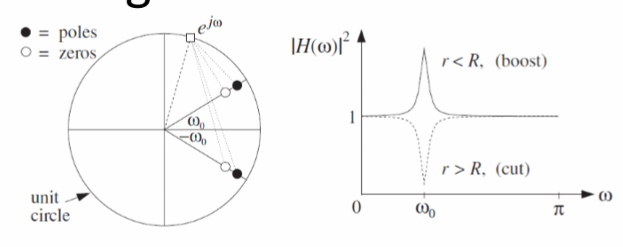
\includegraphics[width=0.8\columnwidth]{Images/general_resonators}
\end{center}

\textbf{Notch Filter}\script{S248-S253}
Bei setzten von Nullen auf dem Einheitskreis $r=1$ ergibt sich
\begin{align*}
	a_1 = Rb_1, &\qquad a_2 = R^2b_2
\end{align*}
\[
H(z) = \frac{1 + b_1z^{-1} + b_2z^{-2}}{1 + Rb_1z^{-1} + R^2b_2z^{-2}} = \frac{N(z)}{N(R^{-1}z)}
\]
\begin{center}
	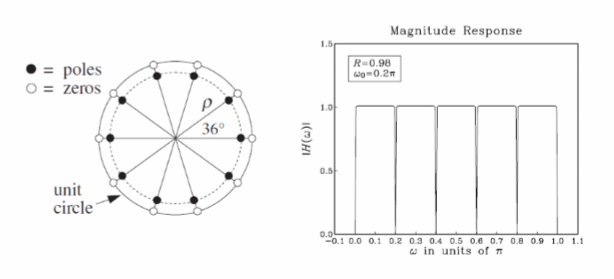
\includegraphics[width=\columnwidth]{Images/notch}
	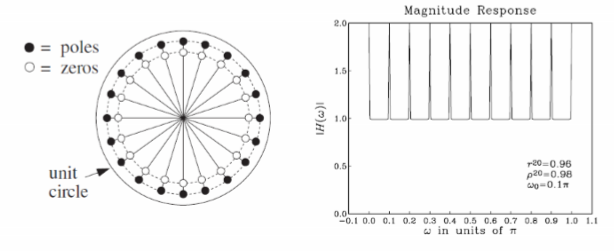
\includegraphics[width=\columnwidth]{Images/notch2}
\end{center}

\subsection{Inverse Filter}\script{S254}
\[
H_{inv}(z) = \frac{1}{H(z)}
\]
Dabei werden Pole und Nullen getauscht. Dabei muss beachtet werden, dass das antikausale Filter nun im $D$ Samples verschoben werden muss. Dies kann zu einer Approximation des Inverse Filters führen.

